\documentclass{beamer}
\bibliographystyle{amsalpha}
\usepackage{cite}
\usepackage[normalem]{ulem}
\usepackage{fancybox}
\usepackage{enumitem}
\setitemize{label=\usebeamerfont*{itemize item}
\usebeamercolor[fg]{itemize item}
  \usebeamertemplate{itemize item}}
\setbeamertemplate{footline}[frame number]{}
\setbeamertemplate{navigation symbols}{}
\graphicspath{{figures/}}

\title{Initializing MD with Prime Numbers}
\author[Price and Shohet]{Jake Price and Michael Murillo}
\institute[CPSSW]{Computational Physics Student Summer Workshop}
\date{\today}

\begin{document}
	\begin{frame}
		\titlepage
	\end{frame}
	
%	\begin{frame}[t]{Outline}
%		\tableofcontents
%	\end{frame}
	

	
	\begin{frame}{The Problem With MD Initialization}
	\begin{columns}
	\begin{column}{0.5\textwidth}
			\begin{itemize}
			\vspace{1em}
			\item In 2003, Michael noted a real-world example of a phenomenon well known to those who run molecular dynamics simulations
			\end{itemize}\vspace{2em}
			
			\includegraphics[width=\linewidth]{disorderinducedheating.eps}
			
			\end{column}
			\begin{column}{0.6\textwidth}
			\includegraphics[width=\linewidth]{disorderinducedheating.png}\vspace{4em}
			\begin{itemize}
			\item Ions placed in a domain at random tend to heat up once the simulation begins!
			\end{itemize}
			\end{column}
			\end{columns}
	\end{frame}
	
	\begin{frame}{The Problem With MD Initialization}
	\begin{itemize}
	\item A random sampling method does not take into account particle correlations that exist in the systems we are trying to simulate
	\vspace{0.5em}
	\item By random chance, two particles will be placed far closer to one another than the potential would typically allow
	\vspace{0.5em}
	\begin{itemize}
	\item Once the simulation begins, they rocket off in opposite directions, driving up the variance of the velocity distribution (aka the temperature)
	\end{itemize}
	\end{itemize}
	
	\begin{center}\includegraphics[width=0.4\linewidth]{happyparticles.png}\end{center}
	\end{frame}
	
	\begin{frame}{The Problem With MD Initialization}
	\begin{itemize}
	\item A random sampling method does not take into account particle correlations that exist in the systems we are trying to simulate
	\vspace{0.5em}
	\item By random chance, two particles will be placed far closer to one another than the potential would typically allow
	\vspace{0.5em}
	\begin{itemize}
	\item Once the simulation begins, they rocket off in opposite directions, driving up the variance of the velocity distribution (aka the temperature)
	\end{itemize}
	\end{itemize}
	
	\begin{center}\includegraphics[width=0.4\linewidth]{unhappyparticles.png}\end{center}
	\end{frame}
	
	
	\begin{frame}{One Solution}
	\begin{itemize}
	\item The solution: thermostats!\vspace{0.5em}
	\begin{itemize}
	\item Langevin\vspace{0.5em}
	\item Nos\'e-Hoover\vspace{0.5em}
	\item Velocity rescaling \vspace{0.5em}
	\item Many more\vspace{0.5em}
	\end{itemize}
	\item Thermostats nudge the velocity distribution toward the desired distribution\vspace{0.5em}
	\item This ``mellows out'' the wild velocities you introduced with your random initialization
	\end{itemize}
	\end{frame}
	
	
	\begin{frame}{Another Solution}
	\begin{itemize}
	\item Initialize the distribution more intelligently\vspace{1em}
	\end{itemize}
	\hspace{1em}Pseudo-random initialization\hspace{4em}Halton initialization
	\begin{center}\includegraphics[width=0.5\linewidth]{random.png}\includegraphics[width=0.5\linewidth]{halton.png}
	
	\tiny (I wonder how many papers today should have Stack Exchange or Wikipedia as a co-author)\end{center}
	

	\end{frame}
	
	
	\begin{frame}{The Halton Sequence}
	\begin{itemize}
	\item The Halton sequence is a deterministic way to select points in a unit square that is low-discrepancy \vspace{0.5em}
	\begin{itemize}
	\item Low-discrepancy means, in layman's terms, that the proportion of points in a sequence that fall in a set $B$ is proportional to the measure of $B$\vspace{0.5em}
	\item Restated, the distribution of points is roughly uniform
	\end{itemize}
	\end{itemize}
	\end{frame}
	
	\begin{frame}{The Halton Sequence}
	\begin{itemize}
	\item The algorithm for a Halton sequence of points filling the unit $n$-dimensional hypercube: \vspace{0.5em}
	\begin{itemize}
	\item For every dimension, select a prime number $a$, divide the interval by $a$ and record, then divide the interval by $a^2$ and record all non-repeating values, and so on up to $N$
	\vspace{0.5em}
	
\item Pair the first element of each sequence for the coordinates of particle 1, and so on up to $N$ particles
	\end{itemize}
	
	\end{itemize}
\begin{center}	\begin{tabular}{|l|c|c|c|c|c|c|c|}\hline
	Prime number &1 &2&3&4&5&6&7\\\hline
	Two & 1/2 & 1/4 & 3/4 & 1/8 & 3/8 & 5/8 & 7/8\\ \hline
	Three & 1/3 & 2/3 & 1/9 & 4/9 & 7/9 & 2/9 & 5/9\\ \hline
	\end{tabular}\end{center}
	Coordinates: $\left(\frac{1}{2},\frac{1}{3}\right)$, $\left(\frac{1}{4},\frac{2}{3}\right)$, $\left(\frac{3}{4},\frac{1}{9}\right)$, $\left(\frac{1}{8},\frac{4}{9}\right)$, $\left(\frac{3}{8},\frac{7}{9}\right)$, $\left(\frac{5}{8},\frac{2}{9}\right)$, $\left(\frac{7}{8},\frac{5}{9}\right)$
	\end{frame}
	
	
	\begin{frame}{The Halton Sequence}
	\begin{itemize}
	\item This sequence has been used to optimize Monte-Carlo integration\vspace{0.5em}
	\item One problem encountered in this application is that the Halton sequence for larger primes have undesired levels of correlation\vspace{0.5em}
	\begin{itemize}
	\item A solution is to independently permute the Halton sequence of each dimension before pairing them as coordinate points
	\vspace{0.5em}
	
\item But is this something we should worry about when using the Halton sequence to initialize MD?\vspace{0.5em}
	\end{itemize}
	\end{itemize}
	
	\end{frame}
	
	\begin{frame}{Answer to Rhetorical Question}
	\begin{center}\huge NO!\end{center}
	\begin{itemize}
	\item When we initialize MD, we do not know the particle-particle correlations, and we use the thermostat phase to allow the system to find its correlation 
	\vspace{0.5em}
	\begin{itemize}
\item The Halton sequence allows us to guarantee no particles accidentally start so close as to artificially spike the temperature\vspace{0.5em}
\item But it also allows us to intelligently select an initial correlation that is close to the desired correlation\vspace{0.5em}
\end{itemize}
\item With a well-selected set of primes, we can initialize with a Halton sequence that makes the thermostat's job as easy as possible
	\end{itemize}
	
	\end{frame}
	
	
	
	
	\begin{frame}{Different Initializations}
	\begin{center}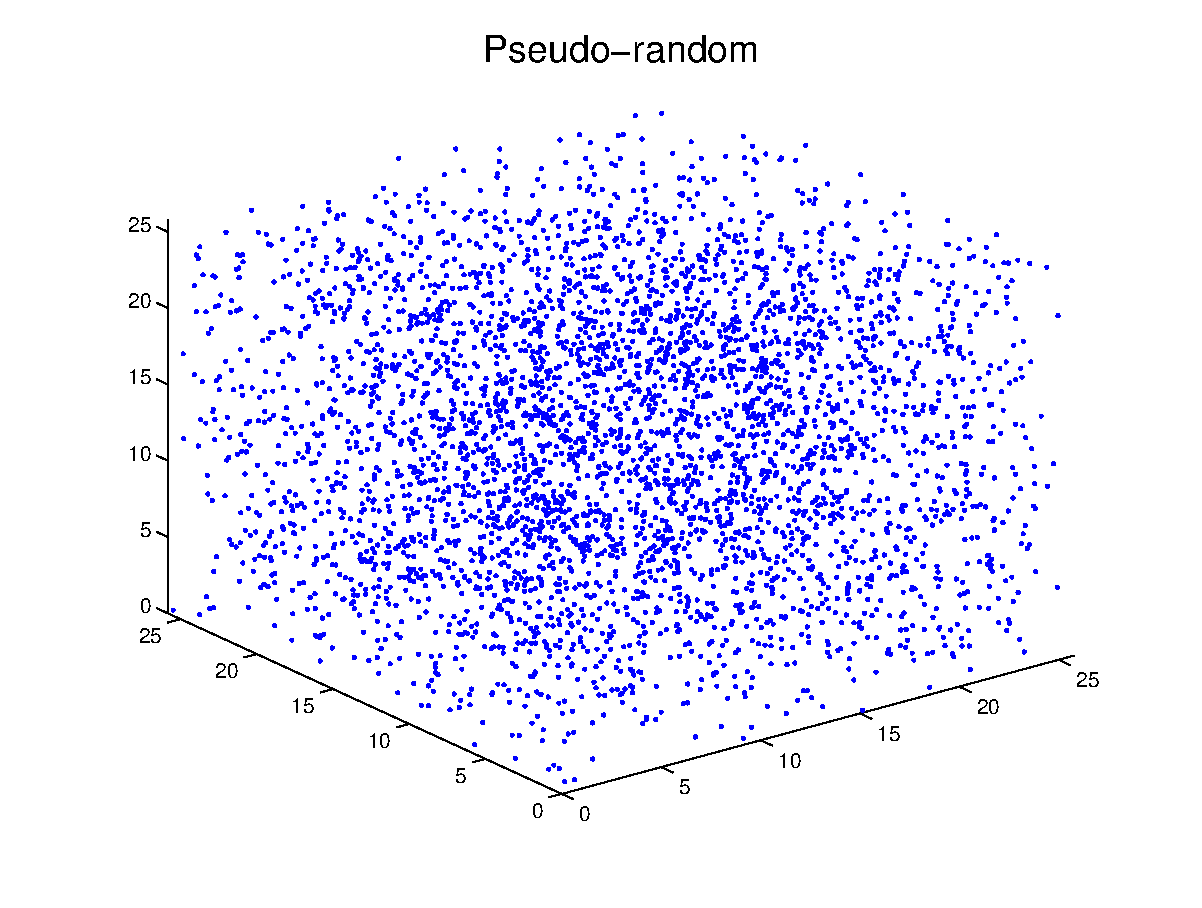
\includegraphics[width=\linewidth]{uniformscatter.eps}\end{center}
	
	\end{frame}
	
	\begin{frame}{Different Initializations}
	\begin{center}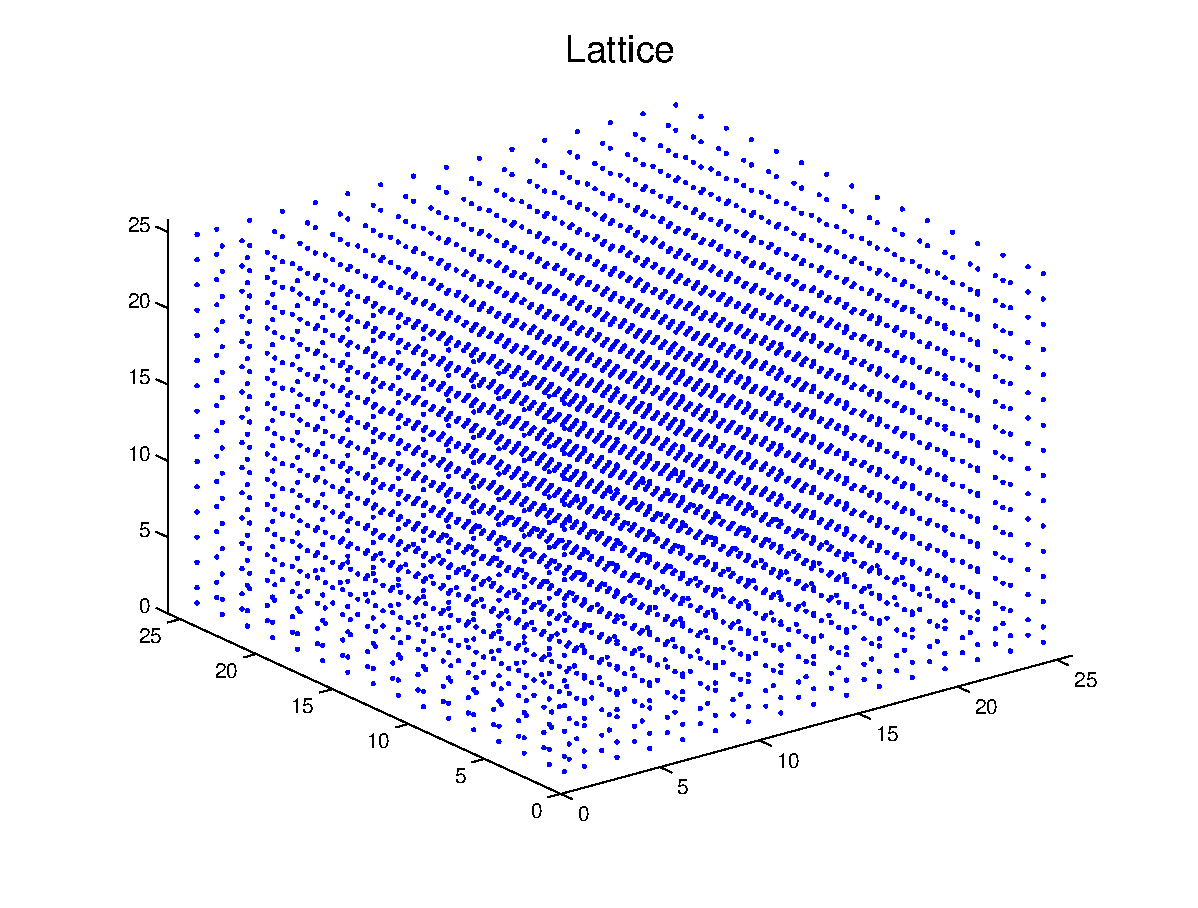
\includegraphics[width=\linewidth]{gridscatter.eps}\end{center}
	
	\end{frame}
	
	
	\begin{frame}{Different Initializations}
	\begin{center}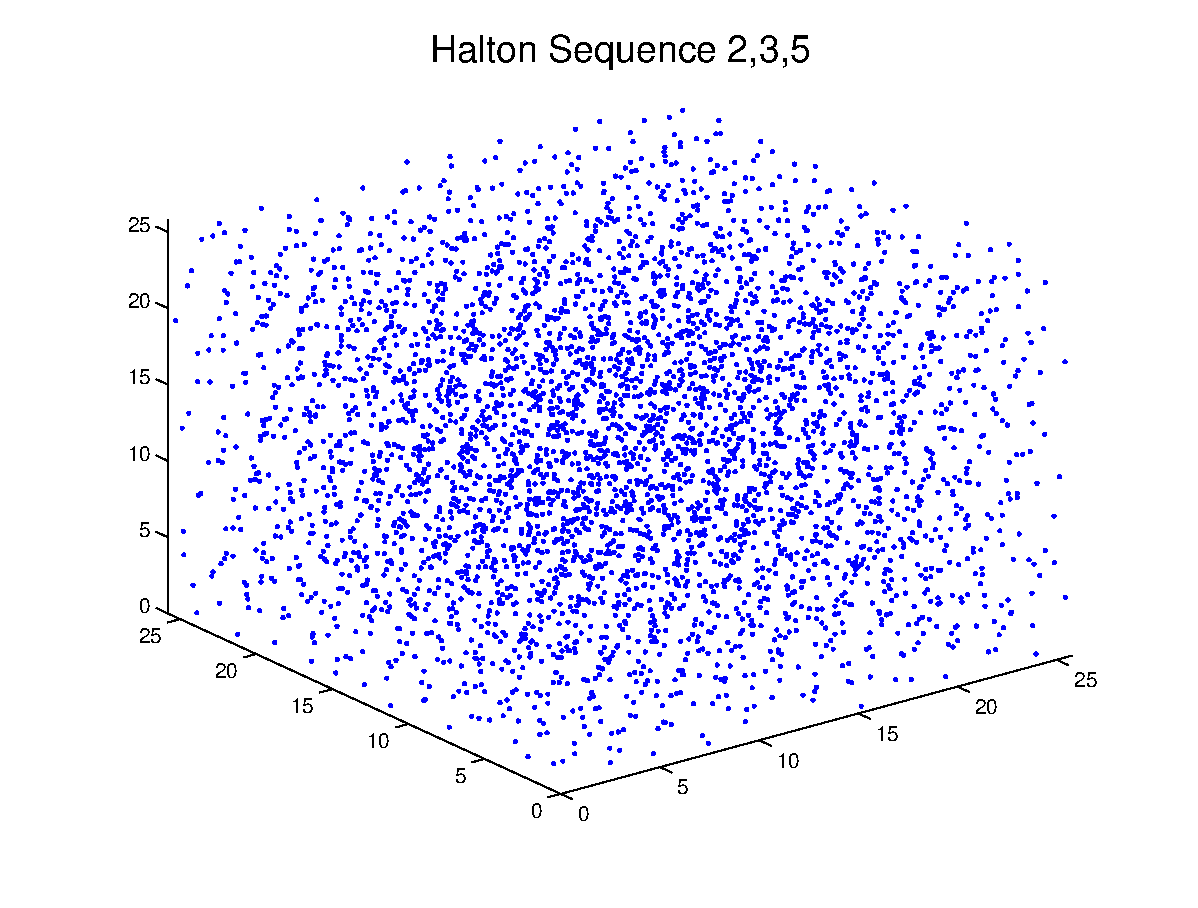
\includegraphics[width=\linewidth]{haltonscatter.eps}\end{center}
	
	\end{frame}
	
	\begin{frame}{Order-Induced Cooling}
	\begin{itemize}
	\item The complete disorder of a pseudo-random initialization inevitably leads to heating as the particles correlate amongst themselves, as described by Michael\vspace{0.5em}
	\begin{itemize}
	\item ``Disorder-Induced Heating''
	\end{itemize}\vspace{0.5em}
	\item A highly ordered system, such as a lattice, inevitably leads to cooling as the particles de-correlate\vspace{0.5em}
	\begin{itemize}
	\item ``Order-Induced Cooling''
	\end{itemize}\vspace{0.5em}
	\item A Halton sequence, depending on the choice of prime numbers, has different levels of correlation\vspace{0.5em}
	\begin{itemize}
	\item Depending on how much it needs to decorrelate, the system will cool different amounts depending on the primes used for each dimension
	\end{itemize}
	
	\end{itemize}
	\end{frame}
	
	
	 

	\begin{frame}{Order-Induced Cooling}\begin{columns}
    \column{\dimexpr\paperwidth-12pt}
	\begin{center}\includegraphics[width=1\linewidth]{kappa1OIC.eps}\end{center}
	 \end{columns}
	\end{frame}
	
	\begin{frame}{Summary}
	\begin{itemize}
	\item These results are preliminary
	\vspace{1em}
	\item If the level of correlations of Halton sequences with different choices of prime numbers are known, and the rough target particle correlations are known, we can imagine initializing at a distribution that minimizes the thermostat time\vspace{1em}
	\item There are many other low-discretion sequences that merit study as possible MD initializations as well
	\end{itemize}
	
	\end{frame}
	
	\begin{frame}{References}
	\nocite{*}
		\bibliography{OIC_bib}
	\end{frame}

\end{document}